\documentclass[border=10pt]{standalone}
\usepackage{fontspec}
\usepackage{unicode-math}
\setmainfont{PT Sans}
\setmathfont[Path=../, math-style=upright]{Neo Euler.otf}
\usepackage{tikz,pgfplots}
\pgfplotsset{compat=1.17}
\usetikzlibrary{positioning,arrows.meta,calc,decorations.pathreplacing,shapes.geometric}
% палитра manim (3Blue1Brown): оттенки A (светлый) ... E (тёмный); линии — D/E, заливки — A
\definecolor{mBlueA}{HTML}{C7E9F1}
\definecolor{mBlueB}{HTML}{9CDCEB}
\definecolor{mBlueC}{HTML}{58C4DD}
\definecolor{mBlueD}{HTML}{29ABCA}
\definecolor{mBlueE}{HTML}{236B8E}
\definecolor{mTealA}{HTML}{ACEAD7}
\definecolor{mTealB}{HTML}{76DDC0}
\definecolor{mTealC}{HTML}{5CD0B3}
\definecolor{mTealD}{HTML}{55C1A7}
\definecolor{mTealE}{HTML}{49A88F}
\definecolor{mGreenA}{HTML}{C9E2AE}
\definecolor{mGreenB}{HTML}{A6CF8C}
\definecolor{mGreenC}{HTML}{83C167}
\definecolor{mGreenD}{HTML}{77B05D}
\definecolor{mGreenE}{HTML}{699C52}
\definecolor{mYellowA}{HTML}{FFF1B6}
\definecolor{mYellowB}{HTML}{FFEA94}
\definecolor{mYellowC}{HTML}{F7D96F}
\definecolor{mYellowD}{HTML}{F4D345}
\definecolor{mYellowE}{HTML}{E8C11C}
\definecolor{mGoldA}{HTML}{F7C797}
\definecolor{mGoldB}{HTML}{F9B775}
\definecolor{mGoldC}{HTML}{F0AC5F}
\definecolor{mGoldD}{HTML}{E1A158}
\definecolor{mGoldE}{HTML}{C78D46}
\definecolor{mRedA}{HTML}{F7A1A3}
\definecolor{mRedB}{HTML}{FF8080}
\definecolor{mRedC}{HTML}{FC6255}
\definecolor{mRedD}{HTML}{E65A4C}
\definecolor{mRedE}{HTML}{CF5044}
\definecolor{mMaroonA}{HTML}{ECABC1}
\definecolor{mMaroonB}{HTML}{EC92AB}
\definecolor{mMaroonC}{HTML}{C55F73}
\definecolor{mMaroonD}{HTML}{A24D61}
\definecolor{mMaroonE}{HTML}{94424F}
\definecolor{mPurpleA}{HTML}{CAA3E8}
\definecolor{mPurpleB}{HTML}{B189C6}
\definecolor{mPurpleC}{HTML}{9A72AC}
\definecolor{mPurpleD}{HTML}{715582}
\definecolor{mPurpleE}{HTML}{644172}
\colorlet{blue}{mBlueE}
\colorlet{red}{mRedE}
\colorlet{green}{mGreenE}
\colorlet{gold}{mGoldE}
\colorlet{purp}{mPurpleE}
\colorlet{maroon}{mMaroonD}
\colorlet{teal}{mTealE}
\colorlet{yellow}{mYellowE}
\colorlet{skyblue}{mBlueD}
\colorlet{fillblue}{mBlueA}
\colorlet{fillgreen}{mGreenA}
\colorlet{fillred}{mRedA}
\colorlet{fillgold}{mGoldA}
\colorlet{fillpurp}{mPurpleA}
\colorlet{fillteal}{mTealA}
\definecolor{grey}{RGB}{150,150,150}
\tikzset{
  neuron/.style={circle, draw=black, line width=1.2pt, minimum size=11mm, font=\Large, fill=white, inner sep=1pt},
  block/.style={rectangle, draw=black, line width=1.2pt, minimum height=10mm, minimum width=16mm, font=\Large, fill=white},
  opnode/.style={rectangle, rounded corners=3mm, draw=black, line width=1.2pt, minimum height=9mm, font=\Large, fill=white, inner xsep=8pt},
  edge/.style={line width=1.2pt, -{Stealth[length=2.6mm]}, shorten >=1pt},
  plain/.style={line width=1.2pt},
  thinedge/.style={line width=0.6pt, grey},
  wl/.style={font=\large, fill=white, inner sep=1.5pt},
  lbl/.style={font=\large},
  curve/.style={black, line width=1.6pt},
  curveB/.style={blue, line width=1.6pt},
  curveR/.style={red, line width=1.6pt},
  hollow/.style={fill=white, draw=blue, line width=1.2pt},
  regionR/.style={fill=fillred, fill opacity=0.6},
  regionB/.style={fill=fillblue, fill opacity=0.6},
  sep/.style={green, line width=1.4pt, dashed},
  cell/.style={draw=black, line width=0.8pt, minimum size=8mm, font=\large, inner sep=0pt},
}
\pgfplotsset{
  dlgrid/.style={grid=major, grid style={dashed, gray!30}},
  dlaxis/.style={axis lines=middle, axis line style={line width=1.2pt, -{Stealth[length=2.6mm]}},
    tick style={line width=1pt, black}, ticklabel style={font=\large}, label style={font=\large},
    xlabel style={anchor=north west}, ylabel style={anchor=south east}, clip=false},
  cls0/.style={only marks, mark=*, mark size=4pt, mark options={fill=blue, draw=blue}},
  cls1/.style={only marks, mark=x, mark size=5pt, mark options={draw=red, line width=2.2pt}},
}

\begin{document}
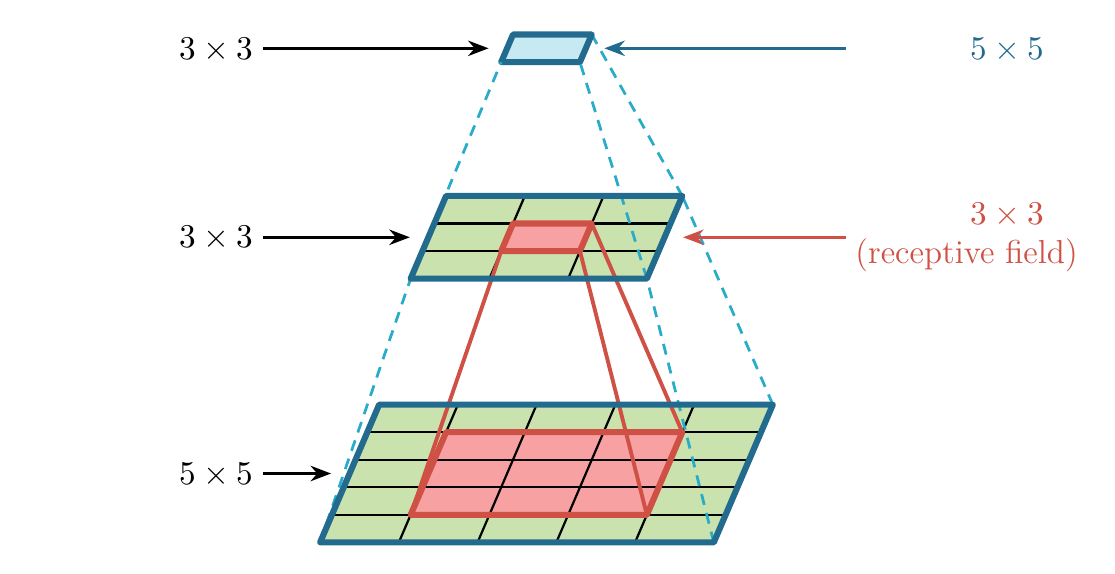
\begin{tikzpicture}[x={(1cm,0cm)}, y={(0.15cm,0.35cm)}, z={(0cm,1cm)}, line join=round]
  \newcommand{\slab}[3]{%
    \fill[fillgreen] (-#2,-#2,#1) -- (#2,-#2,#1) -- (#2,#2,#1) -- (-#2,#2,#1) -- cycle;
    \foreach \t in {#3} {
      \draw[black, line width=0.8pt] (\t,-#2,#1) -- (\t,#2,#1);
      \draw[black, line width=0.8pt] (-#2,\t,#1) -- (#2,\t,#1);
    }}
  \newcommand{\win}[3]{%
    \fill[fillred] (-#2,-#2,#1) -- (#2,-#2,#1) -- (#2,#2,#1) -- (-#2,#2,#1) -- cycle;
    \foreach \t in {#3} {
      \draw[black, line width=0.8pt] (\t,-#2,#1) -- (\t,#2,#1);
      \draw[black, line width=0.8pt] (-#2,\t,#1) -- (#2,\t,#1);
    }
    \draw[red, line width=2.2pt] (-#2,-#2,#1) -- (#2,-#2,#1) -- (#2,#2,#1) -- (-#2,#2,#1) -- cycle;}

  \slab{0}{2.5}{-1.5,-0.5,...,1.5}
  \win{0}{1.5}{-0.5,0.5}
  \foreach \s/\r in {1/1}
    \draw[mBlueD, line width=1pt, dash pattern=on 4pt off 3pt] (2.5*\s,2.5*\r,0) -- (1.5*\s,1.5*\r,3.0);

  \slab{3.0}{1.5}{-0.5,0.5}
  \win{3.0}{0.5}{}
  \draw[red, line width=1.4pt] (1.5,1.5,0) -- (0.5,0.5,3.0);
  \draw[red, line width=1.4pt] (-1.5,-1.5,0) -- (-0.5,-0.5,3.0);
  \draw[red, line width=1.4pt] (1.5,-1.5,0) -- (0.5,-0.5,3.0);
  \foreach \s/\r in {-1/-1, 1/-1}
    \draw[mBlueD, line width=1pt, dash pattern=on 4pt off 3pt] (2.5*\s,2.5*\r,0) -- (1.5*\s,1.5*\r,3.0);
  \foreach \s/\r in {1/1}
    \draw[mBlueD, line width=1pt, dash pattern=on 4pt off 3pt] (1.5*\s,1.5*\r,3.0) -- (0.5*\s,0.5*\r,5.4);

  \filldraw[fill=fillblue, draw=blue, line width=2.2pt] (-0.5,-0.5,5.4) -- (0.5,-0.5,5.4) -- (0.5,0.5,5.4) -- (-0.5,0.5,5.4) -- cycle;
  \foreach \s/\r in {-1/-1, 1/-1}
    \draw[mBlueD, line width=1pt, dash pattern=on 4pt off 3pt] (1.5*\s,1.5*\r,3.0) -- (0.5*\s,0.5*\r,5.4);
  \draw[blue, line width=2.2pt] (-1.5,-1.5,3.0) -- (1.5,-1.5,3.0) -- (1.5,1.5,3.0) -- (-1.5,1.5,3.0) -- cycle;
  \draw[blue, line width=2.2pt] (-2.5,-2.5,0) -- (2.5,-2.5,0) -- (2.5,2.5,0) -- (-2.5,2.5,0) -- cycle;

  \node[lbl, anchor=east] (c2) at (-3.6,0,5.4) {вторая свёртка $3 \times 3$};
  \node[lbl, anchor=east] (c1) at (-3.6,0,3.0) {первая свёртка $3 \times 3$};
  \node[lbl, anchor=east] (c0) at (-3.6,0,0) {картинка $5 \times 5$};
  \draw[edge] (c2.east) -- (-0.7,0,5.4);
  \draw[edge] (c1.east) -- (-1.7,0,3.0);
  \draw[edge] (c0.east) -- (-2.7,0,0);
  \node[lbl, anchor=west, blue] (f2) at (3.8,0,5.4) {поле обзора $5 \times 5$};
  \node[lbl, anchor=west, red, align=left] (f1) at (3.8,0,3.0) {поле обзора $3 \times 3$\\(receptive field)};
  \draw[edge, blue] (f2.west) -- (0.7,0,5.4);
  \draw[edge, red] (f1.west) -- (1.7,0,3.0);
\end{tikzpicture}
\end{document}
